\chapter{性能评估}

为了验证基于软硬协同的中断响应与任务调度设计的有效性,并且评估设计中的各个模块对系统性能的影响,本章在 FPGA 平台上围绕以下三个核心维度展开客观评价:

\begin{itemize}
    \item 任务调度:对基于 TAIC 提供的任务调度功能与传统的软件调度进行多维度对比测试,评估 TAIC 在任务窃取开销等方面的影响;
    
    \item 中断处理:评估基于 TAIC 提供的中断处理机制相较于传统中断处理机制对中断延时的影响;
    
    \item 任务通信:评估基于 TAIC 提供的任务通信能力与传统任务通信机制之间的性能差异。
\end{itemize}

\section{测试环境}

性能评估实验在 ALINX AXU15EG 开发板上展开,该开发板以 Xilinx Zynq UltraScale+ XCZU15EG MPSoC 为核心板,并配备了 DDR4、双千兆以太网接口等外部设备。核心板分为两部分,分别为处理器子系统和可编程逻辑(FPGA)。其中处理器子系统集成了四核 ARM® Cortex-A53 处理器、双核 Cortex-R5 实时处理器,可以直接对开发板上的资源进行控制。FPGA 部分实现了带有 RISC-V N 扩展的 rocket-chip 软核。rocket-chip 软核通过 TileLink 协议与 TAIC 进行交互,并且将 TileLink 协议转换成 AXI 协议来访问 DDR4 内存资源。因此,软核访问 TAIC 与内存的开销相当。

\begin{table}[htbp]
    \centering
    \caption{测试硬件环境}
    \label{tab:platform}
    \begin{tabular}{ll}
        \toprule
        \textbf{IP 核} & \textbf{配置} \\
        \midrule
        \multirow{4}{*}{RISC-V 软核} & rocket chip \\
        & 四核,N 扩展 \\
        & 100MHz 时钟 \\
        & TAIC 中断控制器 \\
        \multirow{2}{*}{以太网} & Xilinx AXI 1G/2.5G 以太网子系统(1Gbps) \\
        & Xilinx AXI DMA \\
        \bottomrule
    \end{tabular}
\end{table}

测试的硬件环境为 FPGA 平台,具体配置如表 \ref{tab:platform}。软件运行于 FPGA 中的 RISC-V 软核上,在微基准测试中,首先测试了软硬件交互接口开销,后续使用了 Linux 6.6.0 版本的基于 RISC-V 指令集的内核进行部分模块的单独测试。而综合测试基于 Rust 语言对 Sel4 \cite{sel4_2025} 重写的 Rel4 微内核 \cite{rel4_kernel} 展开,测试 TAIC 整体功能对应用程序性能的影响。

\section{微基准测试}

微基准测试主要用于从微观层面评估 TAIC 的性能表现。CPU 与 TAIC 之间的交互在几个时钟周期内完成。其中,申请硬件资源需要 4~6 个时钟周期,与任务调度相关的入队/出队操作在 2~4 个时钟周期内完成,与任务通信相关的注册(注销)发送方/接收方以及发送通知的操作在 8~10 个时钟周期内完成。TAIC 接收到中断信号把处于阻塞队列中的任务标识放入到就绪队列中的过程(中断处理),需要 6~8 个时钟周期。除软硬件交互接口测试外,其余测试在Linux 6.6.0 系统环境下完成,具体通过 tokio-bench 和 ipc-bench 两个专业工具展开。

\subsection{任务调度}

tokio \cite{tokio} 作为 Rust 生态中的高性能异步运行时框架,提供了从任务调度到 I/O 操作的全套异步工具链,用于构建高并发、低延时的网络服务。tokio 提供了 rt\_multi\_threaded 基准测试,用于评估多线程环境下的任务调度性能。tokio 的多线程调度器默认使用了任务窃取算法来动态平衡 CPU 上的任务负载,具体的规则如下:

\begin{enumerate}
    \item 针对每个工作线程,单独维护一个有界的局部队列;
    \item 所有的工作线程共用一个无界的全局队列;
    \item \label{item:push_overflow} 当局部队列达到容量上限时,任务将会被放入全局队列中;
    \item \label{item:steal_work}当局部队列没有任务时,工作线程会随机的从其他的工作线程的局部队列中窃取一半的任务;
    \item 当工作线程连续 60 次(tokio 的默认配置)从局部队列中取出任务后,将会从全局队列中取出一个任务。
\end{enumerate}

\begin{figure*}[htbp]
    \centering
    \begin{minipage}[c]{0.32\textwidth}
		\centering
		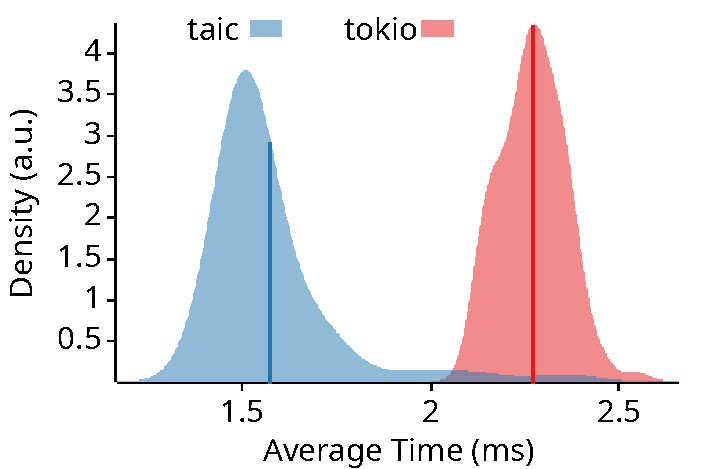
\includegraphics[width=\textwidth]{figures/tokio/chained_spawn.pdf}
		\subcaption{chained\_spawn}
		\label{tokio_chained_spawn}
	\end{minipage}
    \begin{minipage}[c]{0.32\textwidth}
		\centering
		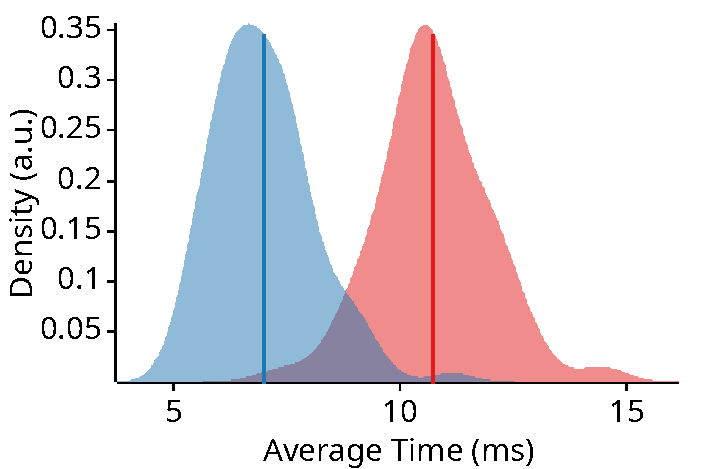
\includegraphics[width=\textwidth]{figures/tokio/spawn_local.pdf}
		\subcaption{spawn\_local}
		\label{tokio_spawn_local}
	\end{minipage}
    \begin{minipage}[c]{0.32\textwidth}
		\centering
		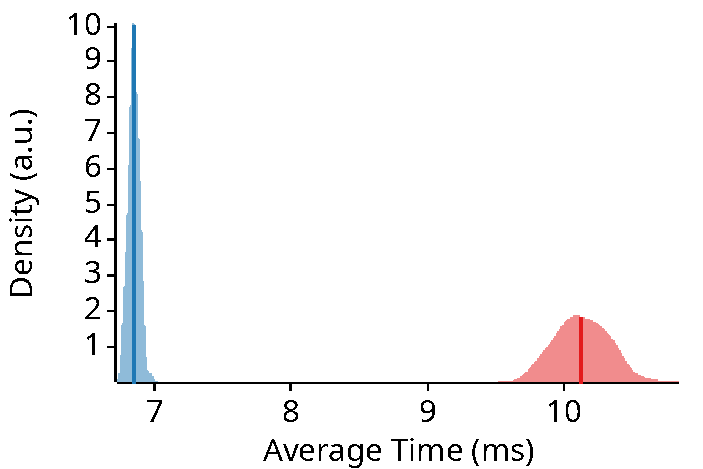
\includegraphics[width=\textwidth]{figures/tokio/spawn_remote_idle.pdf}
		\subcaption{spawn\_remote\_idle}
		\label{tokio_spawn_remote_idle}
	\end{minipage}

    \begin{minipage}[c]{0.32\textwidth}
		\centering
		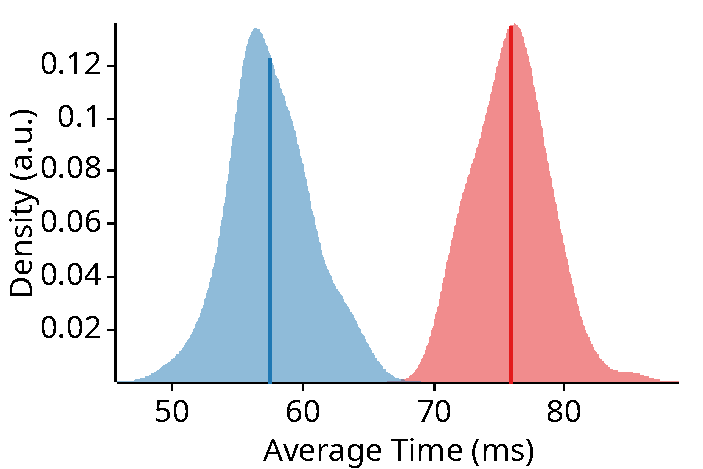
\includegraphics[width=\textwidth]{figures/tokio/yield.pdf}
		\subcaption{yield}
		\label{tokio_yield}
	\end{minipage}
    \begin{minipage}[c]{0.32\textwidth}
		\centering
		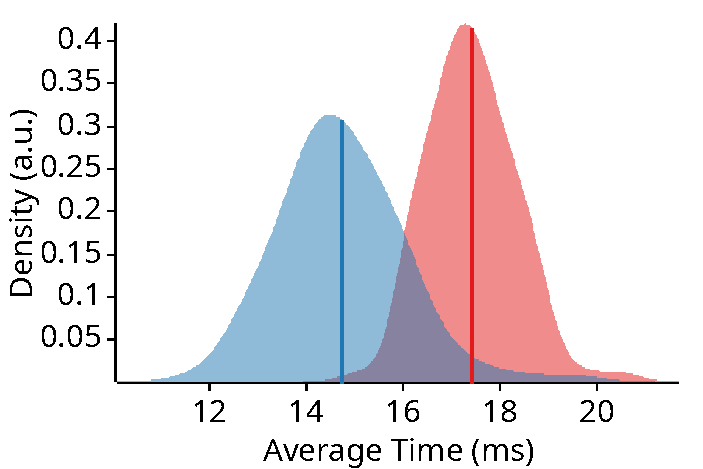
\includegraphics[width=\textwidth]{figures/tokio/ping_pong.pdf}
		\subcaption{ping\_pong}
		\label{tokio_ping_pong}
	\end{minipage}
    \begin{minipage}[c]{0.32\textwidth}
		\centering
		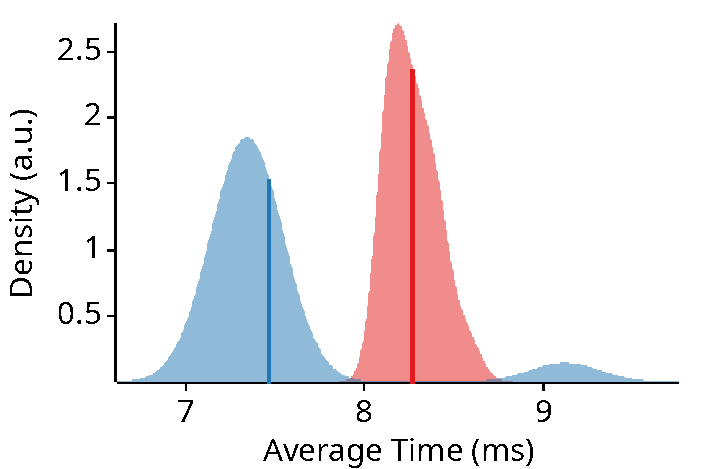
\includegraphics[width=\textwidth]{figures/tokio/spawn_remote_busy.pdf}
		\subcaption{spawn\_remote\_busy}
		\label{tokio_spawn_remote_busy}
	\end{minipage}
    \caption[任务调度对比]{任务调度对比。其中 taic 表示使用硬件任务队列,tokio 表示使用软件任务队列。}
    \label{figure:tokio-bench}
\end{figure*}

本文对 tokio 默认的多线程调度器进行了修改,将其任务窃取算法中使用的任务队列替换为 TAIC 提供的硬件任务队列。每个工作线程使用 TAIC 提供的硬件局部队列,这些硬件局部队列共同构成一个硬件全局队列,如图 \ref{figure:ready_queue} 所示。由于硬件的局部队列没有固定的容量限制,但其最大容量不超过全局队列的容量,因此修改后的 tokio 任务调度器无法满足规则 \ref{item:push_overflow},为了保证公平,测试过程中保证了不会出现局部队列溢出的情况。此外,由于硬件提供了局部队列之间的负载均衡功能,当局部队列中没有任务时,会自动从其他的局部队列中取出任务,因此,规则 \ref{item:steal_work} 也不再需要,但保留了计算随机数的开销来保证测试的公平性。使用上述修改后的 tokio 调度器来评估 TAIC 在任务调度方面的性能表现,最终的结果如图\ref{figure:tokio-bench}所示。

\textbf{任务窃取}:chained\_spawn 测试递归的生成任务,任意时刻,至多存在两个任务,当一个工作线程运行任务 $A$ 生成一个新的任务 $B$ 时,其他的空闲的工作线程会窃取新生成的任务 $B$ 来执行,循环这个过程,直到结束。因此两个测试的性能差异主要取决于任务窃取的性能。taic 在任务窃取时直接从局部队列中可以窃取出其他的局部队列中的任务,而 tokio 原本的软件任务窃取需要搜索开销以及局部队列的同步互斥等额外开销,从图 \ref{tokio_chained_spawn} 可以看出,taic 使得任务窃取的开销下降了 30.68\%。同理,spawn\_local 测试生成更多的任务,并将任务放入当前工作线程的局部队列中,尽管 tokio 原本的任务窃取会直接从其他局部队列中窃取一半的任务,但 taic 提供的硬件任务窃取功能几乎是零开销的,因此,taic 在 spawn\_local 测试(图\ref{tokio_spawn_local})中仍然将任务窃取的开销下降了 34.88\%。spawn\_remote\_idle 测试(图\ref{tokio_spawn_remote_idle})与 spawn\_local 测试类似,不同之处在于它将生成的任务放到了远端队列(远端队列等价于局部队列,用于任务窃取)中,两者的性能差距仍然来源于任务窃取的开销(32.41\%)。

\textbf{任务切换}:yield(图 \ref{tokio_yield})、ping\_pong(图 \ref{tokio_ping_pong}) 和 spawn\_remote\_busy(图 \ref{tokio_spawn_remote_busy}) 测试了在高频任务切换时,硬件任务队列与软件任务队列的性能差异。在 yield 测试中,每个任务在主动让权若干次后结束;在 ping\_pong 测试中,由于相互发送消息的两个任务需要等待对方的消息;在spawn\_remote\_busy 测试中,用户态任务让权后再次运行时,会使用 \verb|sched_yield| 系统调用让当前的工作线程进入内核态让权。因此,使用 taic 节省的任务窃取开销被分摊到每次任务切换以及等待的过程中,使用 taic 将这三个测试的开销分别降低了 24.22\%、15.37\% 和 9.69\%。其中 spawn\_remote\_busy 测试过程中,因为 Linux 内核产生随机数缓慢,导致了使用 taic 时部分测试的平均延时过高。

\subsection{任务通信}

ipc-bench \cite{ipc-bench_2025} 是一个用于测试 Linux 上的包括信号、管道和 eventfd 等 IPC 机制的开源项目。ipc-bench 针对每种 IPC 机制使用了 ping-pong 通信模型(通信双方忙等对方的消息)来测试其性能,性能指标包括通行的总时间、平均每次通信的时间、吞吐量等。

本文参考 ipc-bench 项目中对信号、管道和 eventfd 等 IPC 机制的测试方法,实现了使用 TAIC 进行任务通信的测试程序。测试程序排除了申请 TAIC 硬件资源以及初始化的时间,测试了通信的总时间。其中,所有测试的消息大小为 1 bit,发送消息次数为 1000 次。各项 IPC 机制的性能对比如图 \ref{figure:ipc-bench} 和表 \ref{tab:ipc-bench} 所示。

\begin{figure}
    \centering
    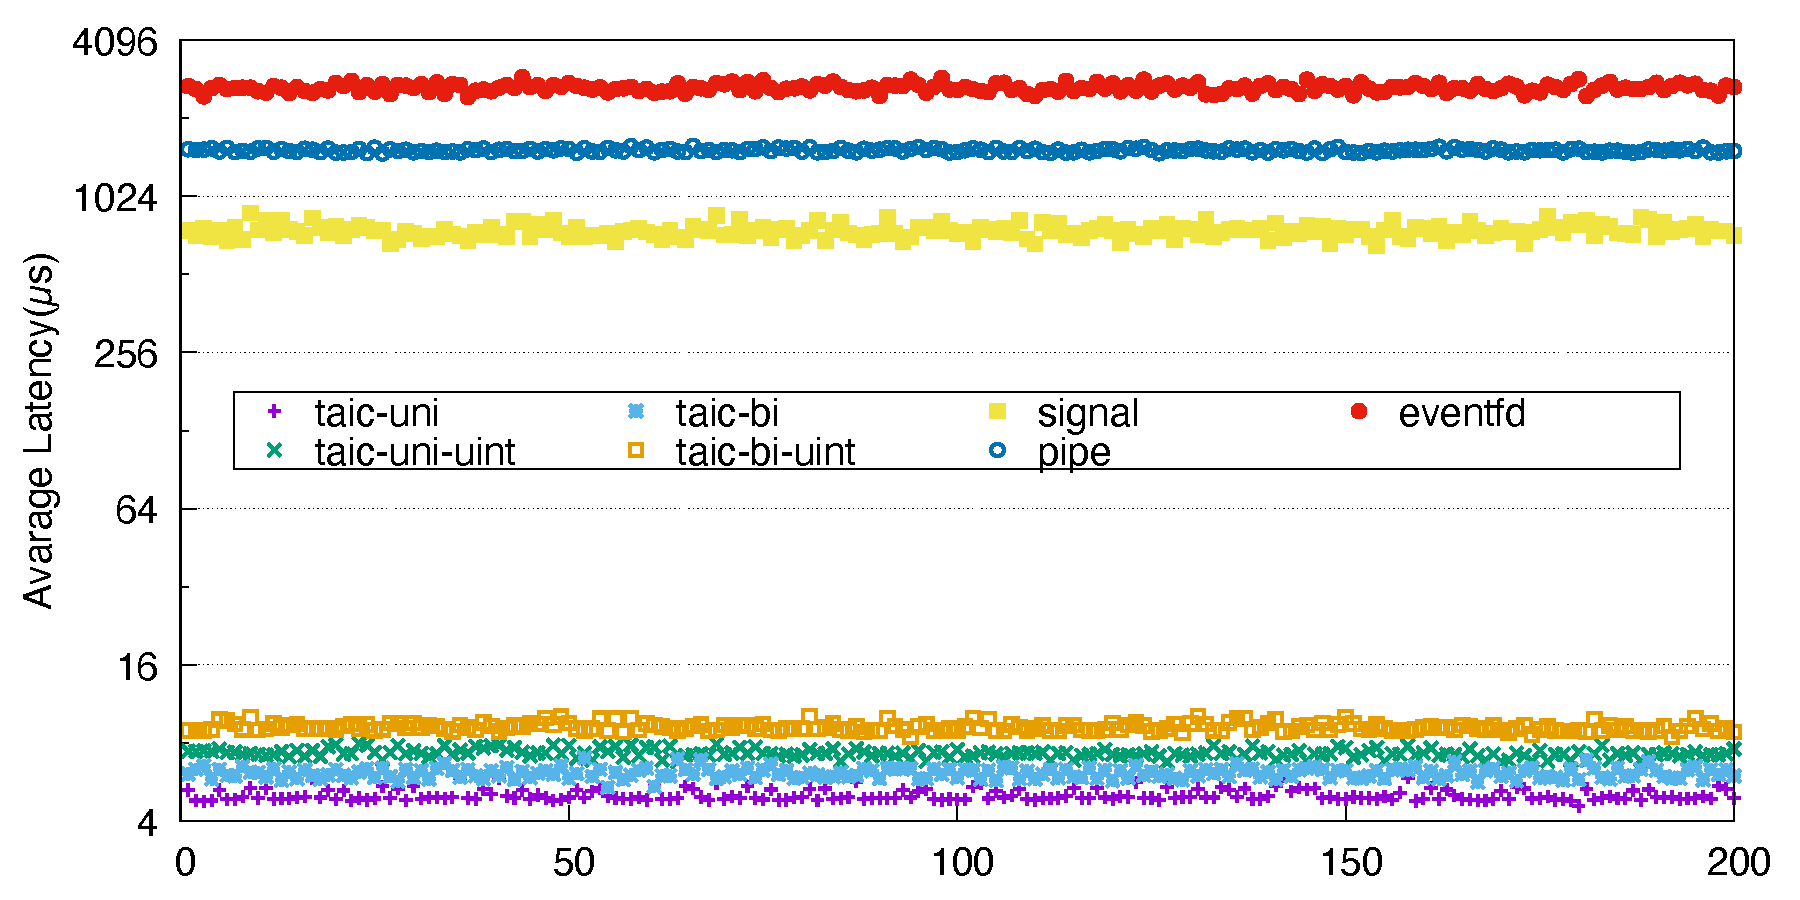
\includegraphics[width=\textwidth]{figures/pdfs/taic-ipc.pdf}
    \caption[IPC 延迟对比]{IPC 延迟对比。taic 表示使用硬件任务通信机制的测试。其中,bi 表示双向,双方互相发送消息;uni 表示单向;uint 表示任务优先级高,需要发送中断。eventfd、pipe、signal 均为双向;}
    \label{figure:ipc-bench}
\end{figure}

\begin{table}
    \centering
    \caption{IPC 性能对比}
    \label{tab:ipc-bench}
    \begin{tabular}{llll}
        \toprule
        \textbf{测试} & \textbf{吞吐量 $msg/s$} & \textbf{平均延时 $\mu s$} & \textbf{相对延迟比} \\
        \midrule
        taic-uni & 199215.0 & 5.02 & 1 \\
        taic-bi & 163158.4 & 6.13 & 1.221 \\
        taic-uni-uint & 137127.0 & 7.29 & 1.453 \\
        taic-bi-uint & 108734.7 & 9.20 & 1.832 \\
        signal & 1334.7 & 749.23 & 149.258 \\
        pipe & 649.6 & 1539.41 & 306.673 \\
        eventfd & 374.9 & 2667.38 & 531.382 \\
        \bottomrule
    \end{tabular}
\end{table}

与 taic 相关的测试保证了通信的接收方在 CPU 上运行(接收方处于在线状态)。不使用中断时,接收方不断尝试从硬件任务队列中取出被唤醒的任务,一旦取出任务则表示收到通知,结束通信的过程;当使用中断时,接收方收到中断信号后,进入用户态的中断的处理逻辑中,从硬件任务队列中取出被唤醒的任务才算收到通知,但需要从中断返回才结束通信;在双向通信中,接收方收到发送方的通知后,向发送方发起通知,直到发送方收到通知才结束通信的流程。

无论是否使用中断来进行任务抢占,使用 TAIC 进行任务通信的性能都远远优于其他的 IPC 机制,在性能上有数量级的提升,能够达到微秒级的时间尺度。但在不使用中断的情况下,若接收方进程正在执行其他的任务,TAIC 内部的中断处理和中断的开销会被其他任务执行掩盖掉,若其他任务的执行时间也处于微秒级,那么即使不需要中断机制,同样可以达到微秒级的通信延迟。

在 ipc-bench 测试的基础上,本文进一步测试了接收方处于不同的特权级的中断延迟(中断延迟包括了 TAIC 中断处理开销、保存被打断任务上下文开销以及软件进行中断分发的开销)。具体的结果如表 \ref{tab:interrupt-latency}所示,括号内表示不包括 TAIC 中断处理开销的中断延迟。结果证明了使用 TAIC 不会增加中断延迟,保证被唤醒的任务可以及时抢占。

\begin{table}
    \centering
    \caption{中断延迟对比}
    \label{tab:interrupt-latency}
    \begin{tabular}{ll}
        \toprule
        \textbf{接收方特权级} & \textbf{CPU 周期} \\
        \midrule
        用户态 & 72(66) \\
        内核态 & 98(92) \\
        \bottomrule
    \end{tabular}
\end{table}

以上的测试没有包括极端的情况。一种极端的情况是接收方运行于用户态,但接收方的进程没有任务在用户态运行,此时,即使唤醒的任务的优先级较高,也无法进行任务抢占,需要等到接收方的进程中存在任务回到用户态运行时才能进行抢占,此时,任务通信的延时除了用户态中断的开销外,还包括了接收方进程等待被调度的时间以及从内核态返回用户态的开销。另一种极端的情况是接收方运行于内核态,但此时接收方没有任务处于内核态运行,因此任务抢占会导致一个正在运行用户态任务的 CPU 陷入内核态,因此任务通信的开销还会包括特权级切换开销(在本文的实验环境下,开销为 870 个时钟周期)。

\section{综合测试}

综合测试在 seL4 微内核环境下展开,评估 TAIC 对 seL4 IPC 机制的性能影响。seL4 作为现代微内核操作系统的代表,它使用同步 IPC 作为进程间通信的主要方式,并且借助需要内核转发的 notification 机制来实现用户态的中断处理和异步通信。然而,seL4 中的同步 IPC 机制会导致大量的上下文切换和二级缓存实效,同时由于阻塞等待,系统无法充分利用多核的性能,导致 seL4 难以满足应用逐渐增加的性能需求。

\subsection{seL4 适配}

本文使用 TAIC 提供的任务通信能力,直接在 seL4 的用户态进程之间构建通信通道,实现用户态异步 IPC 机制,绕过内核的转发,从而减小开销。本文对 seL4 IPC 机制的修改如下:

\begin{itemize}
    \item 收发双方通过共享缓冲区传递消息,实现跨进程的零拷贝数据传递;
    \item 在内核的 notification 对象中维护 TAIC 的资源,增加系统调用,用于用户态进程申请 TAIC 资源;
    \item 用户态进程增加运行时,实现用户态的任务调度以及 IPC 之间的协调;
    \item 收发双方进程使用 TAIC 作为通知机制,并根据共享缓冲区中的标志位实现自适应通知。
\end{itemize}

\begin{figure}[htbp]
    \centering
    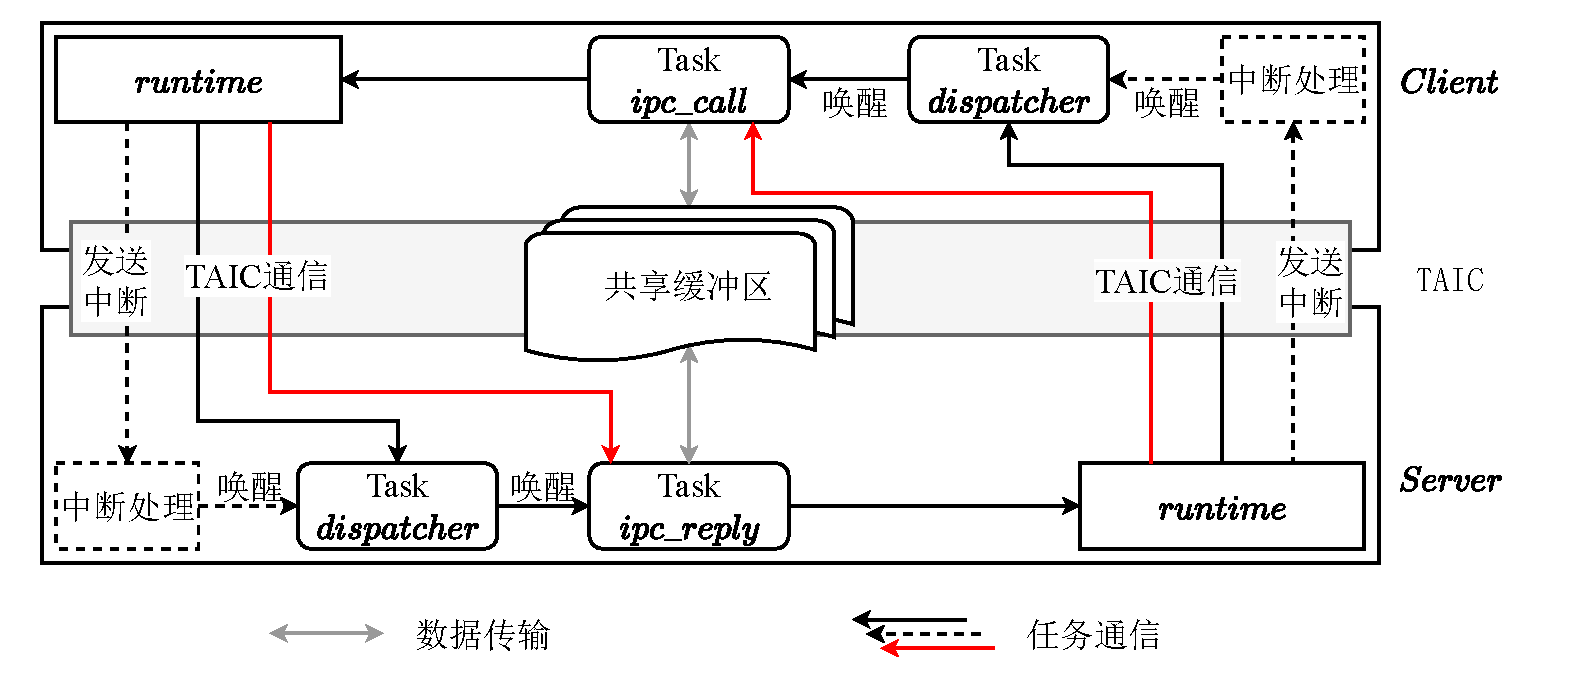
\includegraphics[width=\textwidth]{figures/pdfs/async_ipc.pdf}
    \caption[seL4 异步 IPC 机制]{seL4 异步 IPC 机制}
    \label{figure:seL4_async_ipc}
\end{figure}

以 seL4 IPC 中的 Call 为例,如图 \ref{figure:seL4_async_ipc}。收发双方(客户端进程和服务端进程)由若干个工作(worker)任务和分发(dispatcher)任务共同组成,在双方建立连接时分别注册一个 dispatcher 任务:服务端的 dispatcher 任务读取共享缓冲区中的请求并在处理后将响应结果写入到共享缓冲区中,并根据共享缓冲区中的标志位(表示客户端的 dispatcher 是否处于阻塞状态)判断是否需要通知客户端,当共享缓冲区中没有请求时,它阻塞自己并切换到其他任务;客户端的 dispatcher 任务从共享缓冲区中读取响应结果并唤醒对应的等待的任务,当共享缓冲区中没有响应时,它阻塞自己并切换至其他的任务。IPC 的主要流程分为以下几个阶段:

\begin{enumerate}
    \item 客户端的 worker 任务发起请求:任务根据请求的参数生成存放在共享缓冲区中的请求条目,并且阻塞自己;运行时检查共享缓冲区中的标志位,判断服务端的 dispatcher 任务是否处于阻塞状态,如果服务端的 dispatcher 任务不处于阻塞状态,则无需任何操作;如果 dispatcher 任务处于阻塞状态,那么运行时将共享缓冲区中的标志位清空,并且通过 TAIC 通知服务端的 dispatcher 任务;
    \item 服务端处理请求并写回响应:服务端的 dispatcher 任务从共享缓冲区中读取出请求并分发给对应的处理任务,处理任务将结果写回到共享缓冲区中。运行时检查共享缓冲区中的标志位,如果客户端的 dispatcher 任务不处于阻塞状态,则无需任何操作;否则运行时将标志位清空,通过 TAIC 通知客户端的 dispatcher 任务;
    \item 客户端处理响应:客户端的 dispatcher 任务从共享缓冲区中读取响应并唤醒之前阻塞的任务,然后重启调度。
\end{enumerate}

在上述的 IPC 流程中,TAIC 用于优化通知机制,根据使用的方式,存在以下不同的 IPC 路径:

\begin{itemize}
    \item 使用中断进行唤醒:在这种方式下,收发双方只使用 TAIC 来发送中断信号,使得对方进入用户态中断处理流程,在中断处理中唤醒 dispatcher 任务,即图 \ref{figure:seL4_async_ipc} 中的虚线箭头表示的流程;
    \item 使用 TAIC 任务唤醒:根据唤醒的任务可以进一步划分为两类:(1)唤醒 dispatcher 任务(图 \ref{figure:seL4_async_ipc} 中的黑色箭头流程);(2)直接唤醒 IPC 对应的 worker 任务(图 \ref{figure:seL4_async_ipc} 中的红色箭头流程);
\end{itemize}

\subsection{IPC 性能对比}

为了全方面的评估 TAIC 对于 seL4 IPC 机制的影响,本节在 seL4 中构造了一个服务端进程和客户端进程进行 ping-pong 测试,测量了不同并发量和不同服务端负载下异步 IPC 和同步 IPC的平均开销。测试结果如图 \ref{figure:sel4-ipc-res} 所示。

\begin{figure}
    \centering
    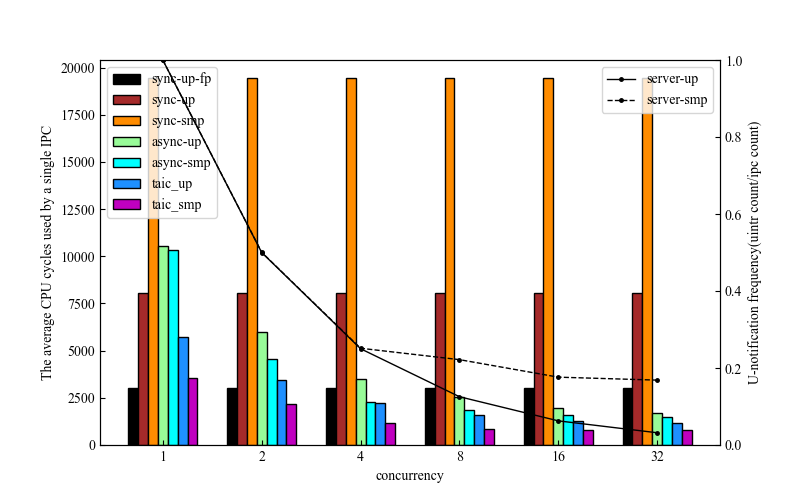
\includegraphics[width=\textwidth]{figures/ipc_test.png}
    \caption[seL4 IPC 性能对比]{seL4 IPC 性能对比。}
    \label{figure:sel4-ipc-res}
\end{figure}

% 由于同步 IPC 会阻塞整个线程,因此并发量对同步 IPC并没有意义。而在多核环境下,seL4 内核的 fast-path 优化机制检查会失败,所有的同步 IPC 都会在内核中通过核间中断进行传递,因此多核环境下的同步 IPC 性能很低;而对于单核下的同步 IPC,fast-path 会避开复杂的消息解码和冗长的调度流程,因此开启 fast-path 的 IPC 性能会提升 167\%,但 fast-path 对于消息长度等有着严苛的检查流程,因此在实际应用场景中 fast-path 优化并不总能生效。

% 从图中的横向比较看,异步 IPC 的开销随着并发量的提升而降低,这是由于随着并发量的增加,服务端的负载进一步增加,dispatcher 任务进入阻塞状态的频率降低,由于采用自适应的形式,因此通知频率下降,导致了均摊到每个 IPC 的开销下降。我们还可以看出,在并发度较小的时候,多核会略快于单核(最高提升 52\%),符合预期,随着并发度的逐渐增加,多核与单核的性能差异逐渐缩小(17\%),这是由于多核情况下服务端单独使用一个 CPU 核心,导致服务端负载过小,产生了更加频繁的用户态中断(如左图中的蓝色折线),导致服务端吞吐量过小,又反过来限制了客户端的请求频率。可以从第二幅图中看出,当我们增加服务端负载时,服务端的中断频率会逐渐下降,直至归 0,这是自适应轮询带来的优势。

% 对比同步 IPC 和异步 IPC,当并发度为 1 的时候,每个异步 IPC 的开销都包含了两次用户态中断的开销、调度器的运行时开销,而同步 IPC 则是两次特权级切换的开销,如果没有 fast-path 优化,还会有内核路径中的解码开销和调度开销,因此在低并发度的场景下异步 IPC 的性能会略低于没有fast-path 优化的同步 IPC(31\%),同时显著低于有 fast-path优化的同步 IPC(249\%)。而当并发量较大时,用户态中断的频率减少,均摊到每一次 IPC 下,用户态中断的开销几乎可以忽略不计,因此异步 IPC 的开销主要是调度器的运行时开销,而此时的异步 IPC 性能会显著高于没有 fast-path 优化的同步 IPC(369\%),也高于有 fast-path 优化的同步 IPC(76\%)。

% 从上面我们可以得出结论:在多核场景下,我们的异步IPC 相比于同步始终有着良好的表现。而在单核且低并发度场景下,异步 IPC 性能会比较差,但随着并发度增加,异步IPC 的性能会迅速提升,在并发度为 2 时就已经超过没有fast-path 优化的同步 IPC,在并发度为 8 时就已经超过了开启 fast-path 优化的同步 IPC,因此异步 IPC 依然十分有竞争力。

% 从上面我们可以得出结论:异步 IPC 在实际应用场景中有利于多路复用的实现,可以有效减少特权级切换的开销,提升系统的整体性能。

\section{本章小结}

本章从任务调度、中断处理以及任务通信三个维度展开对 TAIC 的评估。在微基准测试和综合测试的结果来看,使用 TAIC 提供的软硬件协同能力进行优化后的系统相较于基于传统机制的系统,性能取得了明显的提升,进一步验证了基于软硬协同的中断响应和任务调度机制的有效性。
